\documentclass[tikz]{standalone}
\usepackage{tikz}
\usepackage[AutoFakeBold=true,AutoFakeSlant=true]{xeCJK}
\usepackage[zihao=-4,UTF8,heading=true]{ctex}
\usepackage[simplified]{pgf-umlcd}
\usetikzlibrary{fit} %形状
\usetikzlibrary{positioning} %不加方向运算可能出错
\usetikzlibrary{arrows.meta} %箭头
\usetikzlibrary{calc}

\setCJKmainfont{微软雅黑}
\begin{document}
	\thispagestyle{empty}
    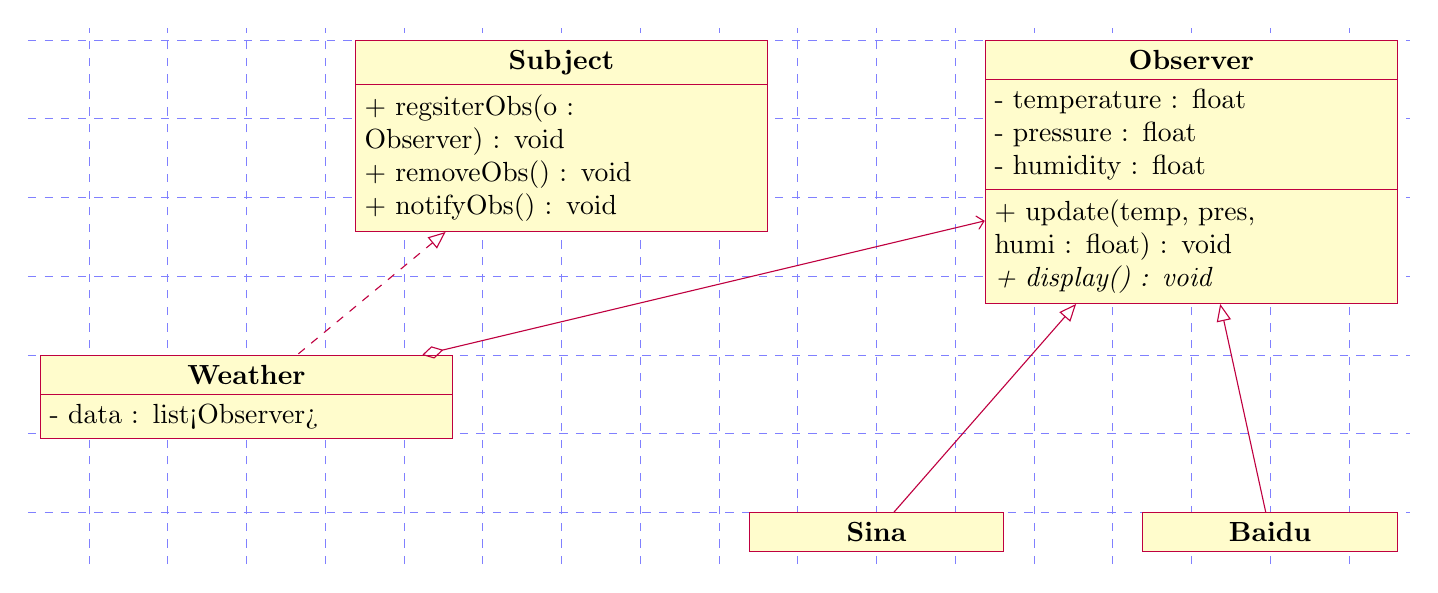
\begin{tikzpicture}[show background grid]
        \begin{class}[text width=5cm]{Subject}{0,0}
            \operation{+ regsiterObs(o : Observer) : void}
            \operation{+ removeObs() : void}
            \operation{+ notifyObs() : void}
        \end{class}
        \begin{class}[]{Weather}{-4, -4}
            \implement{Subject}
            \attribute{- data : list<Observer> }
        \end{class}
        \begin{class}[]{Observer}{8, 0}
            \attribute{- temperature : float }
            \attribute{- pressure : float }
            \attribute{- humidity : float}
            \operation{+ update(temp, pres, humi : float) : void }
            \operation[0]{+ display() : void}
        \end{class}
        \begin{class}[text width = 3cm]{Sina}{4, -6}
            \inherit{Observer}
        \end{class}
        \begin{class}[text width = 3cm]{Baidu}{9, -6}
            \inherit{Observer}
        \end{class}
        \aggregation{Weather}{}{}{Observer}
    \end{tikzpicture}

\end{document}